
\begin{frame}
\frametitle{Adaptive Mesh Refinement for solving PDEs}
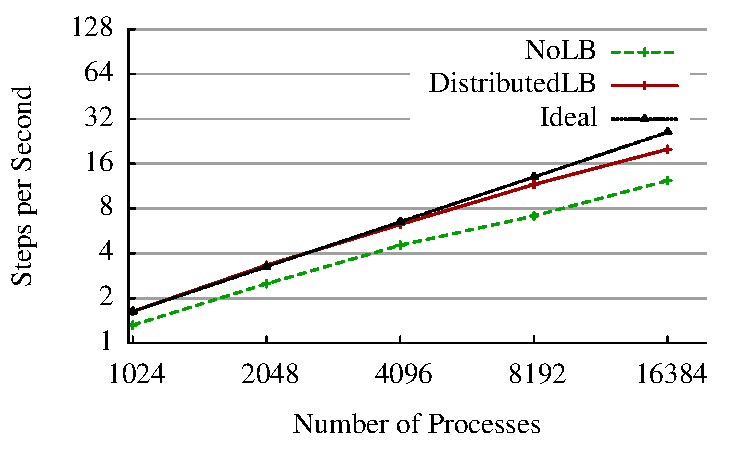
\includegraphics[width=0.9\textwidth]{../figures/amr_scaling_distlb.pdf}
\end{frame}




\begin{frame}[fragile]
\frametitle{Crack Propagation}
\begin{columns}
\begin{column}{0.5\textwidth}
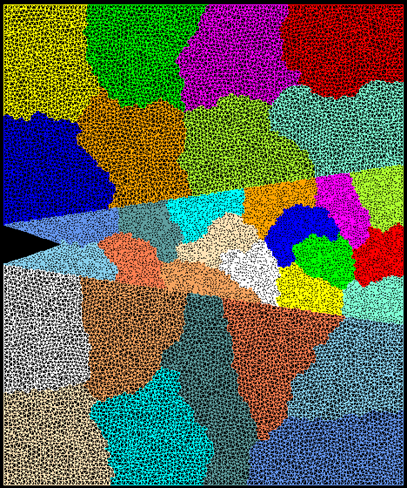
\includegraphics[width=\textwidth]{../figures/chunkGraph16}
\end{column}
\begin{column}{0.5\textwidth}
Decomposition into 16 chunks using Metis. The middle area contains cohesive elements.

As computation progresses, crack propagates, and new elements are added, leading to more complex computations in some chunks

Picture: S. Breitenfeld and P. Geubelle
\end{column}
\end{columns}
\end{frame}

\begin{frame}[fragile]
\frametitle{Load Balancing Crack Propagation}
\begin{centering}
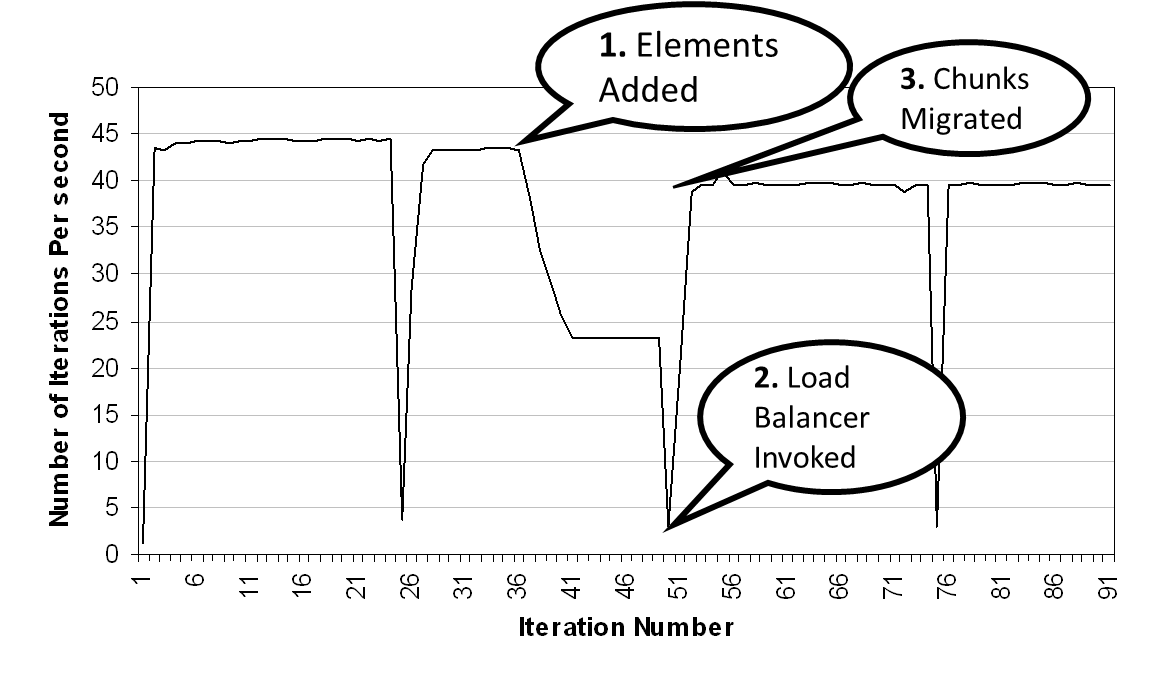
\includegraphics[width=1.0\textwidth]{../figures/LButilizationCrackPropWithAnnotation}
\end{centering}
\end{frame}

